\chapter{Framework for Workload-Aware Teaching Allocation}

%  Integrated Framework for Faculty Workload Aware Teaching Allocation

This section describes how the different areas of research come together to define the allocation framework. It goes on to present a diagram of the framework in \autoref{fig:system_architecture}.

\section{Formal Teaching Workload Allocation}

Formal Teaching Workload allocation refers to allocation of courses, tutorials and labs to individual faculty while keeping their preferences and constraints in mind.

\subsection{Teaching Workload Weightage Calculator}

This involves using the findings in \autoref{chapter:rts_ratio} and \autoref{section:distributing_formal_workload} to calculate the teaching workload that should to be allocated to a faculty, while taking into account the faculty's role, their research and service duties, while also keeping in mind the max workload that can be allocated to a faculty due to practical considerations.

\subsection{Lecture Splitter}

This involves applying the insights from \autoref{chapter:lecture_splitting} into splitting the lectures on the basis of class size and other factors, with the aim of distributing the workload equitably while also keeping the impact of one particular course on a faculty low.

\subsection{Course Weightage Calculator}

This involves applying the insights and calculation methodology from \autoref{section:defining_formal_workload} to calculate the weightages for lectures, tutorials and labs of each course while making considerations for class size, course newness and faculty-course familiarity which affect the amount of work required for them.

\subsection{Faculty Course Matcher}

This involves applying the factors described in \autoref{section:allocation_criteria} to define the most appropriate faculty for a course and condensing these factors into weightages that can be directly used to by the allocation algorithm. Studies have pointed to the biases that student feedback suffers from, including language, accent, racial and gender preferences. However, not all such biases hold true in rating a faculty's teaching capability. In an attempt to solve this, finding methods to counter such biases is an area that will be explored.

\subsection{Allocation Engine}

This involves using the allocation algorithm taking the inputs provided by the Course Weightage Calculator to allocate the courses on the basis of appropriateness defined by the Faculty Course Matcher, and also meeting the constraints defined by the Teaching Workload Weightage Calculator to allocate the courses to faculty while maintaining an optimal and equitable distribution of workload for the faculty.

\section{Informal Teaching Workload Allocation}

Informal Teaching Workload Allocation refers to allocation of FYPs for the faculty on the basis of the workload constraints defined in the Teaching Workload Weightage Calculator, and also taking into consideration the number of Masters' and PhD students under the individual faculty.

\section{Management Insights}

Management Insights gathers statistical insights provided by all the above modules to describe the overall allocation quality in factors such as-
\begin{itemize}
    \item Fulfilment of organizational goals
    \item Equity and outliers in the workload distribution of faculty
    \item Gaps in faculty expertise which result in aforementioned outliers
    \item Overdependence on certain faculty members
\end{itemize}

\section{Framework diagram and Research Timeline}

The diagram gives a high-level view of the submodules, inputs, and outputs of the allocation framework. The diagram after describes the timeline for completion of the research.

\begin{sidewaysfigure}
    \centering
    \scalebox{.16}{\includegraphics{images/overview.png}}
    \caption{Overview of the system architecture}
    \label{fig:system_architecture}
\end{sidewaysfigure}

\begin{sidewaysfigure}
    \centering
    \scalebox{0.9}{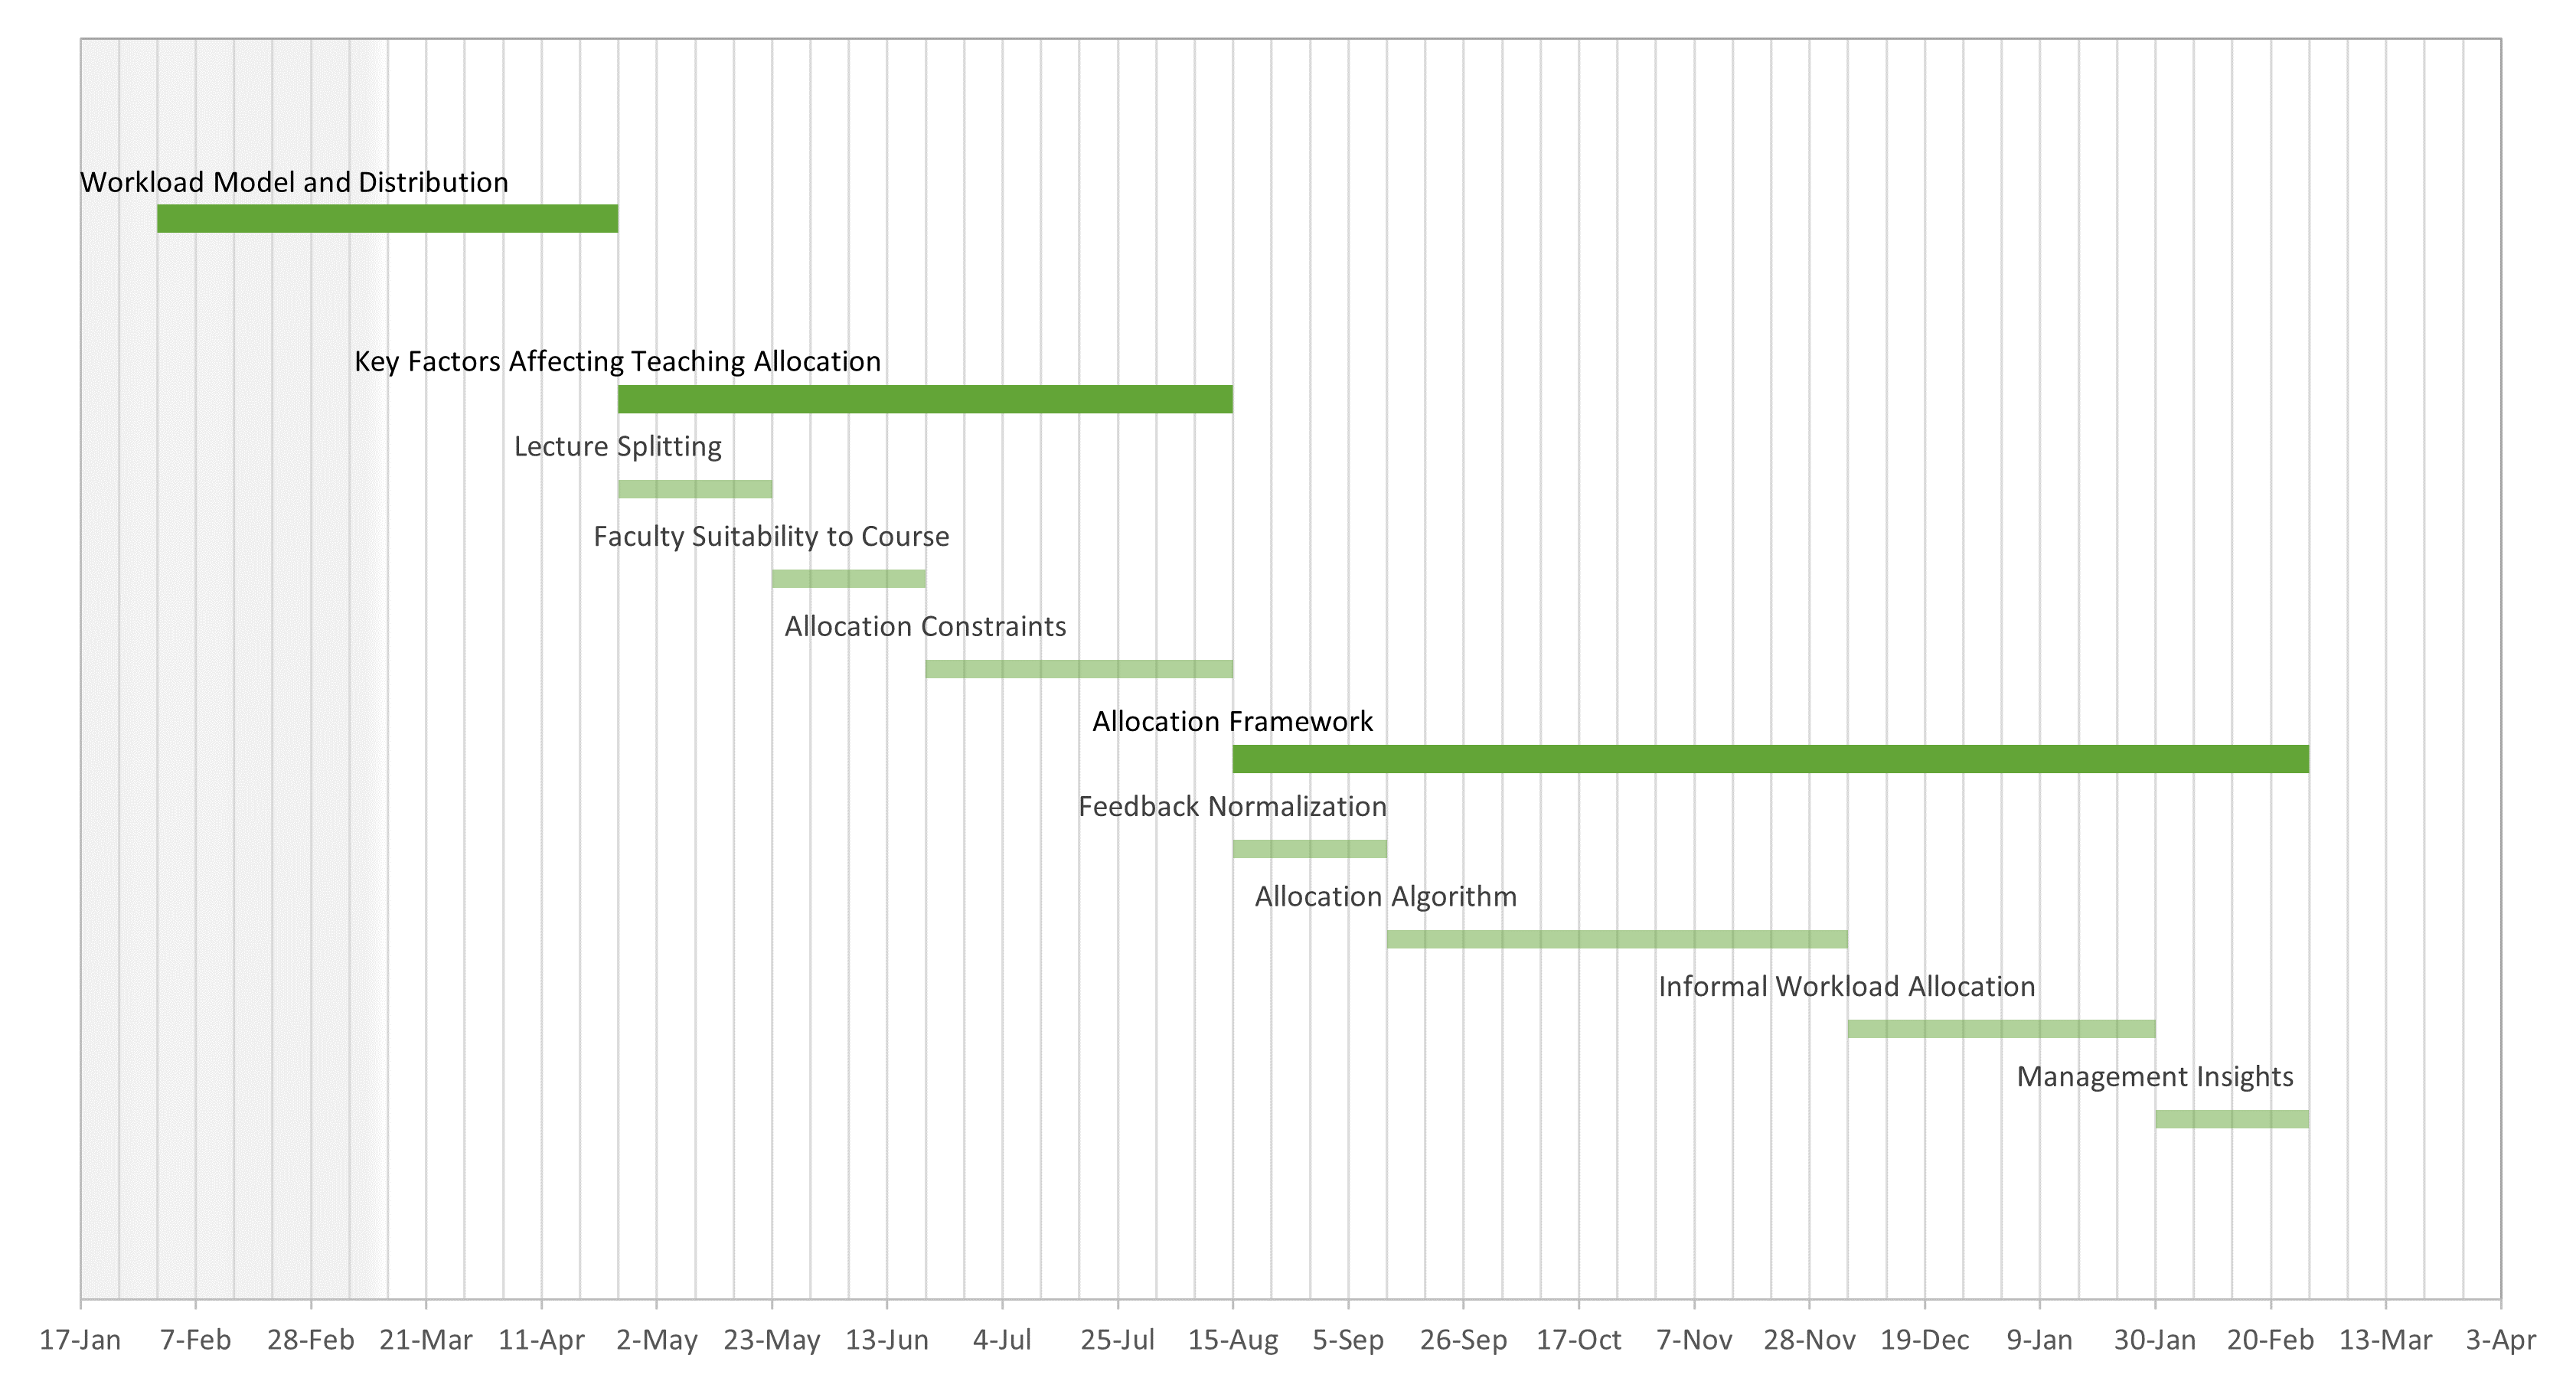
\includegraphics{images/gantt_chart.png}}
    \caption{Research Timeline plan}
    \label{fig:gantt_chart}
\end{sidewaysfigure}
